\documentclass[
	% -- opções da classe memoir --
	12pt,				% tamanho da fonte
	openright,			% capítulos começam em pág ímpar (insere página vazia caso preciso)
	oneside,			% para impressão em frente e verso. Oposto a oneside
	a4paper,			% tamanho do papel.
	% -- opções da classe abntex2 --
	chapter=TITLE,		% títulos de capítulos convertidos em letras maiúsculas
	%section=TITLE,		% títulos de seções convertidos em letras maiúsculas
	%subsection=TITLE,	% títulos de subseções convertidos em letras maiúsculas
	%subsubsection=TITLE,% títulos de subsubseções convertidos em letras maiúsculas
	% -- opções do pacote babel --
	english,			% idioma adicional para hifenização
	french,				% idioma adicional para hifenização
	spanish,			% idioma adicional para hifenização
	brazil				% o último idioma é o principal do documento
	]{abntex2}
% ---
% Pacotes básicos 
% ---
\usepackage{lmodern}			% Usa a fonte Latin Modern
\usepackage{mathptmx}			% Usa a fonte Times New Roman
\usepackage[T1]{fontenc}		% Selecao de codigos de fonte.
\usepackage[utf8]{inputenc}		% Codificacao do documento (conversão automática dos acentos)
\usepackage{lastpage}			% Usado pela Ficha catalográfica
\usepackage{indentfirst}		% Indenta o primeiro parágrafo de cada seção.
\usepackage{color}				% Controle das cores
\usepackage{graphicx}			% Inclusão de gráficos
\usepackage{subcaption}				% Inclusão de gráficos lado a lado
\usepackage{microtype} 			% para melhorias de justificação
\usepackage{tabularx,ragged2e}	% Para inserir tabelas
\usepackage{multirow}			% Para mesclar células
\usepackage[dvipsnames,table,xcdraw]{xcolor}		% Permite adicionar cores nas linhas de tabelas
\usepackage{fancyvrb}			% Permite adicionar arquivos de texto
\usepackage[portuguese, ruled, linesnumbered]{algorithm2e} % Uso de algoritmos
\usepackage{amsfonts}			% Permite usar notação de conjuntos
\usepackage{amsmath}			% Permite citar equações
\usepackage{amsthm}				% Permite criar teoremas e experimentos
\usepackage[font={bf, small}, labelsep=endash, labelfont=bf]{caption}	% Faz legenda de figuras ficarem em negrito
\usepackage{cancel}				% Permite fazer expressão tendendo a zero
\usepackage{epstopdf}			% Converte eps para pdf
\usepackage[final]{pdfpages}
\usepackage{hyperref}
\usepackage{fancybox}
\usepackage{float}




\newcolumntype{L}{>{\RaggedRight\arraybackslash}X}
% ---
% ---
% Pacotes adicionais, usados apenas no âmbito do Modelo Canônico do abnteX2
% ---
\usepackage{lipsum}				% para geração de dummy text
% ---
% ---
% Pacotes de citações
% ---
%\usepackage[brazilian,hyperpageref]{backref}	 % Paginas com as citações na bibl
\usepackage[alf, abnt-emphasize=bf]{abntex2cite}	% Citações padrão ABNT
% ---
% Customizações para o layout da UFPA
% ---
\usepackage{modelo-ufpa/ufpa}
% Muda o título de lista de ilustrações para lista de figuras
\addto\captionsbrazil{%
  \renewcommand{\listfigurename}%
    {Lista de Ilustrações}%
	\renewcommand{\listtablename}%
    {Lista de Tabelas}%
}
% Permite utilizar figuras sem precisar colocar o caminho absoluto
\graphicspath{{imagens/}}
% Define o ambiente de experimentos
\theoremstyle{definition}
\newtheorem{experimento}{Experimento}[section]
\newcommand{\experimentoautorefname}{Experimento}


% --------------------------------------------------------------
% Informações do TRABALHO
% --------------------------------------------------------------
\universidade{UNIVERSIDADE FEDERAL DO PARÁ}
\instituto{INSTITUTO DE TECNOLOGIA}
\faculdade{FACULDADE DE COMPUTAÇÃO E TELECOMUNICAÇÕES}
%\curso{CURSO DE BACHARELADO EM SISTEMAS DE INFORMAÇÃO}
\titulo{RELATÓRIO DE SISTEMAS OPERACIONAIS}
\autor{
%\begin{tabular}{l l}
    DAVID PINHEIRO DE SOUSA - 202207040045 \\
    JOAO VICTOR SANTOS BRITO FERREIRA - 202207040028 \\
    JOEL TAVARES MIRANDA - 202206840054 \\
    KAUAN MIRANDA TAVARES - 202206840033 \\
    MARCO ANTONIO DO ESPIRITO SANTO MAUES JUNIOR - 202206840038 \\
%\end{tabular}
}
\local{Belém}
\data{2023}
\orientador{Prof. Dr. Diego Lisboa Cardoso}
\tipotrabalho{Monografia}

% o nome da instituição e a área de concentração 
\preambulo{Relatório do trabalho 5 de Sistemas Operacionais.}
%\sobrenome{Sobrenome}
%\nome{Nome}
%\palavraschave
%\datadadefesa{Data da Defesa: 09 de Março de 2017}%07 de Dezembro de 2016}
\conceito{Conceito: Excelente}
\faculdadedoorientador{Faculdade de Biotecnologia - UFPA}
\primeiromembrodabanca{Prof. Dr. Nome Sobrenome}
\faculdadedoprimeiromembrodabanca{Faculdade de Computação - UFPA}
\segundomembrodabanca{Prof. Dra. Nome Sobrenome}
\faculdadedosegundomembrodabanca{Faculdade de Biotecnologia - UFPA}
% -------------------------------------------------------------------------
% ---
% Configurações de aparência do PDF final
% alterando o aspecto da cor azul
\definecolor{blue}{RGB}{41,5,195}
% informações do PDF
\makeatletter
\hypersetup{
     	%pagebackref=true,
		pdftitle={\imprimirtitulo}, 
		pdfauthor={\imprimirautor},
    	pdfsubject={\imprimirpreambulo},
	    pdfcreator={LaTeX with abnTeX2},
		pdfkeywords={\imprimirpalavraschave}, 
		colorlinks=true,       		% false: boxed links; true: colored links
    	linkcolor=black,          	% color of internal links
    	citecolor=black,        		% color of links to bibliography
    	filecolor=magenta,      		% color of file links
		urlcolor=blue,
		bookmarksdepth=4,
        breaklinks=true
}
\makeatother
% --- 
% Espaçamentos entre linhas e parágrafos 
% --- 
% O tamanho do parágrafo é dado por:
\setlength{\parindent}{1.3cm}
% Controle do espaçamento entre um parágrafo e outro:
\setlength{\parskip}{0.2cm}  % tente também \onelineskip
% compila o indice
% ---
\makeindex
% ---

% -------------------------------------------------------------------------
% ---------------------------INICIO DO DOCUMENTO---------------------------
% -------------------------------------------------------------------------
\begin{document}
% Seleciona o idioma do documento (conforme pacotes do babel)
\selectlanguage{brazil}
% Retira espaço extra obsoleto entre as frases.
\frenchspacing 
% ----------------------------------------------------------
% ELEMENTOS PRÉ-TEXTUAIS
% ----------------------------------------------------------
% \pretextual

% ---
% Capa
% ---
\imprimircapa
% ---

% ---
% Folha de rosto

\imprimirfolhaderosto

\newpage

\setlength{\absparsep}{18pt} % ajusta o espaçamento dos parágrafos do resumo

\pdfbookmark[0]{\contentsname}{toc}
\tableofcontents*
\cleardoublepage
% ---
% ---------------------------------------------------------
% ELEMENTOS TEXTUAIS
% ----------------------------------------------------------
\textual

% ----------------------------------------------------------
% Introdução
% ----------------------------------------------------------

\chapter{Introdução}
O sistema de arquivos é uma peça fundamental para o gerenciamento eficiente de dados em 
sistemas operacionais. Entre as diversas opções disponíveis, a escolhida para este trabalho 
foi o sistema de arquivos ext4, ou Quarta Extensão, que destaca-se como uma escolha proeminente para ambientes 
baseados em Linux. Ao longo deste trabalho serão apresentados diversos aspectos, características e benchmarks de desempenho 
do sistema ext4.

\chapter{Apresentação do Sistema}

O Ext4, ou Fourth Extended Filesystem, é uma evolução do sistema de arquivos Ext3, desenvolvido 
especificamente para o sistema operacional Linux. Sua criação foi motivada pela necessidade 
de aprimorar as funcionalidades do Ext3 e acompanhar as demandas crescentes de armazenamento e 
processamento de dados na era moderna da computação. Ao abordar as limitações do Ext3, o Ext4 
oferece uma série de inovações que vão além do seu antecessor.

Com o objetivo de proporcionar um ambiente de armazenamento mais eficiente e confiável, o 
Ext4 introduz melhorias significativas em termos de capacidade, desempenho e segurança. 
Sua arquitetura foi projetada para suportar volumes de dados consideravelmente maiores, 
oferecendo maior flexibilidade para lidar com as demandas crescentes das aplicações contemporâneas. 
Dentre as características e aprimoramentos do Ext4 iremos citar algumas principais como a Retrocompatibilidade,
o Journaling e as evoluções em termo de capacidade, velocidade e tamanho de arquivos.
%Uma característica fundamental do Ext4 é a implementação de registro em diário ("journaling") ilustrado 
%na figura \ref{fig:journaling}, mantendo um registro 
%das operações no sistema de arquivos. Isso permite uma recuperação eficiente durante a inicialização, reduzindo o 
%risco de corrupção de dados em casos de falha do sistema ou desligamento inesperado.


%\section{Retrocompatibilidade}

%Sendo atualmente o Ext3 um dos sistemas de arquivos mais populares em uso pelo Linux, executar a migração para o Ext4 é 
%uma tarefa simples e fácil, pois o Ext4 foi desenvolvido para ser completamente compatível com as demais versões do sistema 
%de arquivos, futuras e antigas (até certo ponto conforme figura \ref{fig:3-4}). A compatibilidade com as futuras versões se deve ao 
%fato de ser possível montar um sistema de arquivos Ext3 da mesma forma que um sistema de arquivos Ext4. Para que seja possível 
%aproveitar todos os benefícios do sistema de arquivos Ext4 é necessária esta migração. Também é possível montar um sistema de 
%arquivos Ext4 como se fosse um sistema de arquivos ext3 (compatibilidade anterior), desde que este não possua extensões.
%\begin{figure}[H]
%	\centering
%	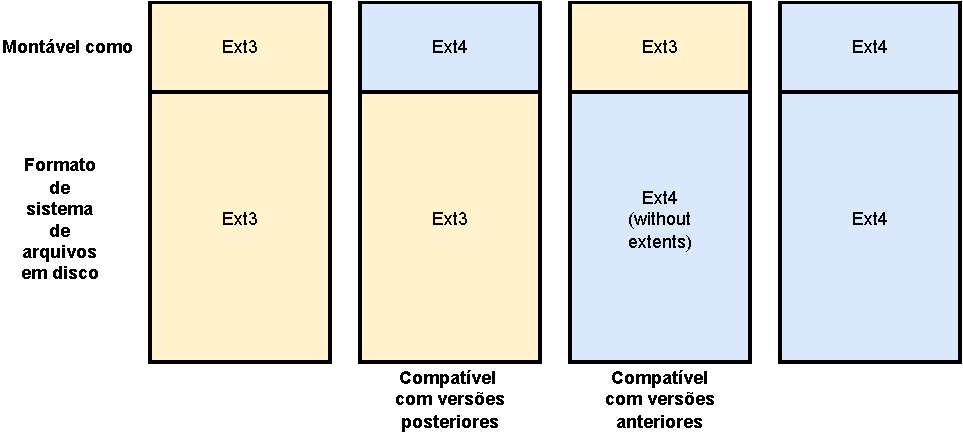
\includegraphics[width=0.95\textwidth]{3-4.pdf}
%	\caption{}
%	\label{fig:3-4}
%\end{figure}
%
%\begin{figure}[H]
%	\centering
%	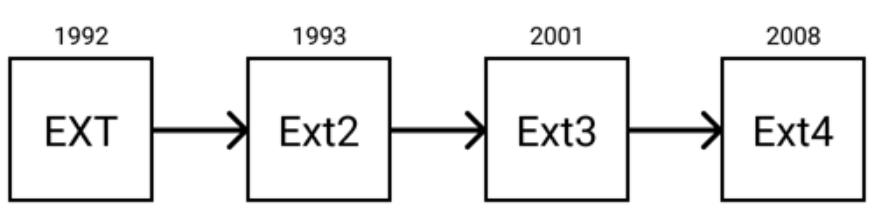
\includegraphics[width=1.0\textwidth]{ext.png}
%	\caption{Cronologia de desenvolvimento do sistema EXT}
%	\label{fig:ext}
%\end{figure}

%\section{Journaling}

%Journaling é o processo de registro de mudanças no sistema de arquivos por meio de um journal (um log circular dedicado em uma região adjacente do disco). As alterações reais no armazenamento físico são então efetuadas partir do log, que pode implementá-las com mais confiabilidade e garantir a consistência, mesmo se houver travamento do sistema ou faltar energia durante a operação. O resultado é que reduzem-se as chances de que o sistema de arquivos seja corrompido.

%Entretanto, mesmo com o journaling, a corrupção ainda será possível se entradas errôneas forem inseridas no diário. Para enfrentar esse problema, o ext4 implementa a verificação de checksum do journal para certificar-se de que as alterações válidas cheguem ao sistema de arquivos subjacente.

%O ext4 oferece suporte a vários modos de journaling, dependendo das necessidades do usuário. Por exemplo, o ext4 oferece suporte a um modo no qual somente metadados são gravados no journal (modo Writeback), um modo no qual os metadados são gravados no journal, mas os dados são gravados como os metadados são gravados a partir do journal (modo Ordenado) e um modo no qual tanto os metadados quanto os dados gravados no journal (modo Journal —o modo mais confiável). Observe que o modo Journal, apesar de ser o melhor para assegurar um sistema de arquivos consistente, também é o mais lento, pois todos os dados passam pelo journal.

%\begin{figure}[H]
%	\centering
%	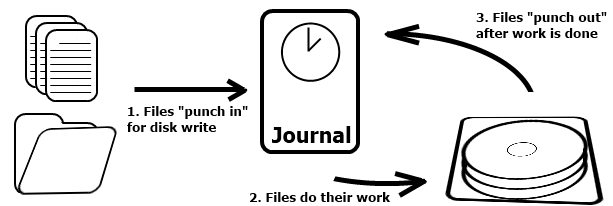
\includegraphics[width=1.0\textwidth]{journaling.png}
%	\caption{heading}
%	\label{fig:journaling}
%\end{figure}

%Uma melhoria significativa do Ext4 em relação ao Ext3 é a introdução do conceito de "extensões". 
%Em vez de manter listas detalhadas de blocos individuais, o Ext4 organiza os dados em extensões, 
%sequências de blocos contíguos. Essa abordagem reduz a fragmentação, melhorando a eficiência do acesso aos dados e otimizando 
%o desempenho do sistema.

%\section{Checksums no Contexto de Sistemas de Arquivos}

%Um checksum, também conhecido como soma de verificação, é uma técnica crucial para garantir a integridade dos dados em sistemas de arquivos. Utilizado para detectar alterações acidentais ou corrupções, os checksums são essenciais para garantir a confiabilidade das informações armazenadas.

%A importância dos checksums reside na capacidade de verificar se os dados permanecem íntegros durante operações de leitura e gravação. Isso é fundamental em ambientes onde a precisão e integridade dos dados são cruciais, como em sistemas de arquivos.

%Diferentes algoritmos de checksum, como MD5, SHA-1 e SHA-256, oferecem diferentes níveis de segurança. A escolha do algoritmo depende dos requisitos específicos de segurança e desempenho do sistema.

%No sistema de arquivos \textit{ext4}, checksums são implementados para verificar a integridade de dados armazenados. Esta funcionalidade é aplicada a vários metadados, incluindo blocos de dados e inodes. A detecção de corrupções contribui para a segurança e confiabilidade do sistema de arquivos.

%Em síntese, a utilização de checksums no sistema de arquivos \textit{ext4} desempenha um papel fundamental na manutenção da integridade dos dados. A escolha cuidadosa do algoritmo e a aplicação abrangente em metadados proporcionam uma camada adicional de segurança, contribuindo para a robustez do sistema de arquivos.


%Além disso, o Ext4 inclui somas de verificação nos metadados do sistema de arquivos, contribuindo 
%para a detecção de corrupção de dados. Essa adição é crucial para melhorar a integridade dos dados 
%armazenados, proporcionando uma camada adicional de segurança e confiabilidade ao sistema de arquivos.

\section{Capacidade, Velocidade e Tamanho de Arquivos}
%Descreva a capacidade do sistema, velocidade e o suporte a arquivos grandes.
A capacidade do sistema de arquivos Ext4 é notavelmente extensa, com um tamanho máximo teórico de 1 exabyte. Essa 
ampla capacidade o torna ideal para lidar com grandes volumes de dados em ambientes Linux, oferecendo suporte a 
sistemas de arquivos significativamente grandes.

Em termos de velocidade, o Ext4 apresenta melhorias significativas em relação ao Ext3, principalmente devido 
à implementação de extensões. Ao organizar os dados em blocos contíguos, o Ext4 reduz a fragmentação, melhorando 
a eficiência no acesso aos dados e otimizando o desempenho global do sistema.

O tamanho máximo do arquivo, aumentado para 16 terabytes, proporciona uma flexibilidade substancial ao lidar 
com arquivos grandes. Essa expansão é crucial em ambientes que exigem o armazenamento e a manipulação de dados 
massivos, garantindo que o Ext4 atenda às demandas de cenários que envolvem arquivos consideravelmente grandes.


\chapter{Sistema de Alocação de Arquivos}
%Explicação sobre como o ext4 aloca arquivos no disco.
No Ext4 o a alocação de arquivos desempenha um papel vital na organização e na gestão eficiente do espaço em disco. 
Dito isso, o Ext4 utiliza uma estrutura aprimorada em comparação aos seus predecessores, Ext2 e Ext3, para otimizaro 
o desempenho e a eficiência,a seguir são apresentados alguns aspectos da alocação no Ext4

%\section{Extensões (Extents)}
%Uma das melhorias significativas introduzidas no Ext4 é o conceito de \textit{extensões} ou \textit{extents}. Em vez de manter listas detalhadas de blocos individuais para armazenar dados de um arquivo, o Ext4 organiza os dados em extensões, que são sequências de blocos contíguos. Essa abordagem ajuda a reduzir a fragmentação do sistema de arquivos, melhorando a eficiência no acesso aos dados.

\section{Alocação por Reservas (Reservation)}
O Ext4 utiliza o conceito de \textit{alocação por reservas} para melhorar o desempenho durante a criação de novos arquivos. Ele reserva espaço em disco antecipadamente para o crescimento futuro do arquivo, evitando a necessidade de buscar continuamente espaço conforme o arquivo cresce. Isso reduz a fragmentação e melhora a eficiência na alocação de espaço.

\section{Alocação por Bloco Indireto}
O Ext4 faz uso de \textit{alocação por bloco indireto} para otimizar a gestão de grandes arquivos. Em vez de armazenar todos os ponteiros diretamente em um bloco, o Ext4 usa uma estrutura de árvore de blocos para referenciar outros blocos, permitindo uma gestão mais eficiente de grandes quantidades de dados.

\section{Tamanho de Bloco Variável}
O Ext4 oferece suporte a \textit{tamanhos de bloco variáveis}, permitindo que os usuários escolham o tamanho de bloco mais adequado às suas necessidades. Isso pode impactar o desempenho e a eficiência na utilização do espaço em disco, dependendo do tipo de dados armazenados.

\section{Alocação Pré-Alocada (Preallocation)}
O Ext4 suporta a \textit{alocação pré-alocada}, onde os aplicativos podem reservar espaço em disco antes de gravar dados. Isso é benéfico em cenários onde a alocação prévia de espaço pode otimizar o desempenho durante a gravação de grandes conjuntos de dados.

\chapter{Gestão do Espaço Livre}
Detalhes sobre como o ext4 gerencia o espaço livre no disco.
%%%%%%%%%%%%%%%%%%%%%%%%%%%%%%%%%%%%%%%%%%%%%%%%%%%%%%%%%%%%%%%%%%%%%%%%%%%%%%%%%%%%%%%%%%%%5

\chapter{Estrutura do Sistema de Arquivos}
%Descrição da estrutura interna do ext4, destacando a organização em grupos de blocos.

O superbloco no Ext4 é bastante semelhante ao de seus antecessores, com a adição de novos campos para 
suportar números de bloco de 64 bits. Até o momento, os campos de carimbo de data e hora no superbloco 
ainda são de 32 bits e não possuem um campo de bits mais significativos associado a eles; no entanto, 
destaca-se que o campo \texttt{s\_log\_groups\_per\_flex} desempenha um papel crucial na organização 
dos grupos de blocos. Nas versões mais recentes do kernel, o superbloco também incorpora campos 
destinados ao rastreamento de erros e à criação de snapshots.

%%%%%%%%%%%%%%%%%%%%%%%%%%%%%

\section{Grupos de Blocos}
O Ext4 mantém estruturas fundamentais, mas introduz diferenças notáveis na organização dos grupos 
de blocos. Um desafio enfrentado é o limite de 128 MB por grupo de blocos, que afeta o tamanho total 
do sistema de arquivos. Duas soluções propostas são o recurso de meta-grupo de blocos e o recurso de 
flex-grupo de blocos.

O meta-grupo de blocos possibilita a criação de meta-grupos compostos por uma série de grupos de 
blocos, todos descritos por um único bloco de descritor. Detalhes adicionais indicam que backups 
dos descritores de meta-grupo de blocos são armazenados no segundo e último grupo de cada meta-grupo de blocos.

A Figura \ref{fig:9} ilustra como o recurso de flex-grupo de blocos estende a ideia anterior 
de criar grandes áreas contíguas de grupos de blocos. Isso é feito movendo os mapas de bits de bloco e 
inode, juntamente com as tabelas de inode, para o primeiro grupo de blocos em um flex-grupo de blocos, 
junto com os descritores de grupo. Com o recurso de superbloco esparsamente ativado por padrão, alguns
grupos de blocos podem conter cópias de backup do superbloco, descritores de grupo e blocos de 
crescimento de descritores de grupo.

\begin{figure}[H]
	\centering
	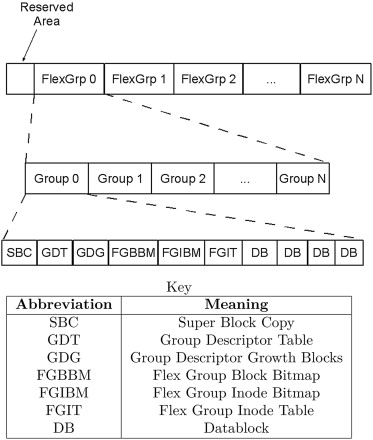
\includegraphics[width=0.36\textwidth]{fig9.jpg}
	\caption{Layout Flexível de Grupos de Blocos}
	\label{fig:9}
\end{figure}

Ao levantar a restrição dos blocos de metadados terem que residir no grupo de blocos ao qual se 
referem, é possível criar um grupo de blocos virtual maior. Isso permite a alocação de blocos de
dados contíguos livres através das fronteiras do grupo. Nas discussões nas listas de desenvolvimento, 
a questão de se as duas opções devem ter diferentes flags de recursos foi abordada. Ficou acordado 
que isso era necessário para manter uma definição clara de \texttt{META\_BG} e \texttt{FLEX\_BG}. 
O recurso \texttt{FLEX\_BG} foi detalhado, pois é selecionado por padrão no arquivo de configuração \texttt{mke2fs}.

\section{Extents (Extensões)}

Outra característica essencial do Ext4 é a adoção de \textit{"extents"} em vez do método de mapeamento 
de blocos previamente utilizado. Os \textit{"extents"} são mais eficientes 
para mapear blocos de dados de arquivos grandes e contíguos, pois sua estrutura inclui o endereço do 
primeiro bloco físico de dados seguido por um comprimento. A Figura \ref{fig:fig10} exibe a estrutura 
do \textit{"extent"} no Ext4, permitindo a sumarização de até 215 blocos com uma única entrada. 
Quando o sistema de arquivos tem um tamanho de bloco de 4 KB, isso mapeia até 128 MB de dados 
com uma única entrada, usando o bit mais alto do campo de comprimento para pré-alocação persistente.

\begin{figure}[H]
    \centering
    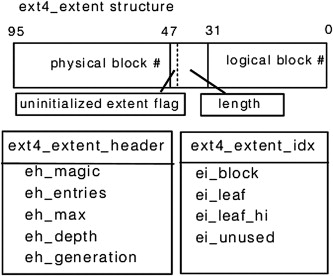
\includegraphics[width=0.5\textwidth]{fig10.jpg}
    \caption{Estrutura do \textit{"extent"} no Ext4 \cite{matur}.}
    \label{fig:fig10}
\end{figure}

De acordo com \cite{matur}, um inode no Ext4 pode conter até quatro \textit{"extents"}. A 
colocação desses \textit{"extents"} no Ext4 é onde anteriormente estavam os ponteiros de bloco no 
Ext3. O formato inclui uma matriz de 60 bytes, com os primeiros 12 bytes contendo um cabeçalho de 
\textit{"extent"}. A estrutura do cabeçalho de \textit{"extent"} é composta pelos campos 
\textit{eh\_magic}, \textit{eh\_entries}, \textit{eh\_max}, \textit{eh\_depth} 
(2 bytes cada) e \textit{eh\_generation} (4 bytes), sendo o número mágico 0xf30A. 
Quando um arquivo é altamente fragmentado, muito grande ou esparsamente distribuído, 
uma árvore de \textit{"extent"} é construída, conforme mostrado na Figura \ref{fig:fig11}.

\begin{figure}[H]
    \centering
    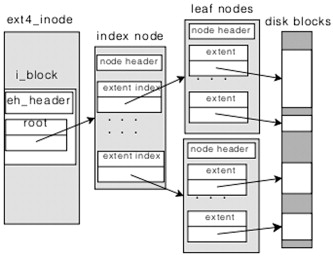
\includegraphics[width=0.5\textwidth]{fig11.jpg}
    \caption{Estrutura da árvore de \textit{"extents"} no Ext4 \cite{matur}.}
    \label{fig:fig11}
\end{figure}

A estrutura de índice 
de \textit{"extent"} atua como uma estrutura intermediária, apontando para um bloco que 
contém outras estruturas que, por sua vez, apontam para dados. Esta estrutura possui um campo
\textit{ei\_block} (4 bytes) usado para denotar o bloco inicial do arquivo ao qual o índice se 
refere. As árvores de \textit{"extents"} válidas devem aderir a regras específicas, 
como a presença do cabeçalho de \textit{"extent"} em cada nó e a ordenação crescente dos 
campos \textit{ee\_block} em nós folha, além do aumento nos valores \textit{ei\_block} em nós de índice.

É importante observar que essas considerações de \textit{"extents"} proporcionam maior eficiência 
no mapeamento de grandes volumes de dados contíguos, oferecendo benefícios significativos ao 
desempenho e à gestão de espaço em disco no Ext4. Para uma visualização mais detalhada dessas 
estruturas, consulte as Figuras \ref{fig:fig10} e \ref{fig:fig11} em \cite{matur}.

\section{Inodes e Tempo no Ext4}

Como observado por \cite{matur} e \cite{xia}, o Ext3 é limitado à resolução de segundos 
no nível do sistema de arquivos. Isso é abordado no Ext4 modificando e estendendo a estrutura de 
inode. Embora o Ext3 suporte tamanhos diferentes de inode que são potências de dois maiores que 128 
bytes até o tamanho de um bloco de sistema de arquivos, 128 bytes é o tamanho padrão. As estruturas 
mais recentes no Ext4 serão, por padrão, de 256 bytes \cite{matur}. Este espaço permite ao 
Ext4 suportar carimbos de tempo em nanossegundos e números de versão de inode de 64 bits. 
Conforme mostrado na Figura \ref{fig:ext4-inode}, os primeiros 128 bytes permanecem em 
grande parte iguais, enquanto os novos campos são adicionados ao final da estrutura. 
Além disso, um novo campo de carimbo de tempo foi adicionado para documentar o momento 
da criação do arquivo. Cada campo de carimbo de tempo no inode, com exceção do carimbo de tempo de 
exclusão, possui um campo de 32 bits correspondente. Nesse espaço, apenas os 30 bits superiores são 
usados para representação em nanossegundos. Os 2 bits restantes são usados como bits mais significativos 
da segunda parte dos carimbos de tempo, adiando assim o problema de 2038 por 272 anos. 
Essa melhoria na resolução de tempo do ponto de vista do sistema de arquivos pode ser 
útil para pesquisas futuras em forense computacional e segurança. O espaço restante é 
ocupado por atributos estendidos rápidos. Nos primeiros 128 bytes, o número de fragmento 
de 1 byte, o tamanho do fragmento de 1 byte e um campo de preenchimento de 2 bytes foram 
substituídos pelos campos \texttt{i\_blocks\_high} e \texttt{file\_acl\_high}, cada um com 16 bits.

\begin{figure}[H]
  \centering
  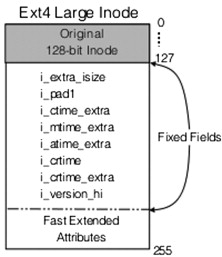
\includegraphics[width=0.4\textwidth]{fig12.jpg}
  \caption{Ext4 inode. Original apareceu em \cite{matur}.}
  \label{fig:ext4-inode}
\end{figure}

Embora o tamanho padrão dos inodes do Ext4 seja de 256 bytes, sistemas de 
arquivos Ext4 podem ser criados com um tamanho de inode de 128 bytes. Nesse caso, os campos 
\texttt{i\_ctime\_extra}, \texttt{i\_mtime\_extra}, \texttt{i\_atime\_extra}, \texttt{i\_crtime}, 
\texttt{i\_crtime\_extra} e \texttt{i\_version\_hi} não estarão presentes. Para os campos 
relacionados a carimbos de tempo, isso resulta nos benefícios mencionados anteriormente de 
suporte a subsegundos, uma extensão de 2 bits para carimbos de tempo e a perda do carimbo de tempo de criação.

Todas as alterações na estrutura de dados afetaram o \textit{journaling}, pois o JBD (Seção 2.2) 
foi ramificado para JBD2, que pode suportar o \textit{journaling} de sistemas de arquivos de 32 bits e 64 bits.

\chapter{Desempenho: Benchmarks}

\section{Teste de Leitura Sequencial}
Resultados e análise do teste de leitura sequencial.

\section{Teste de Escrita Sequencial}
Resultados e análise do teste de escrita sequencial.

\section{Teste de Leitura Aleatória}
Resultados e análise do teste de leitura aleatória.

\section{Teste de Escrita Aleatória}
Resultados e análise do teste de escrita aleatória.

\chapter{Conclusão}
Sumarize os principais pontos abordados no relatório, destacando a adequação do ext4 para os requisitos do trabalho.

\postextual

\bibliography{bibliografia}

\cite{FAIRBANKS2012S118}
\cite{bovet_cesati_2005}
\cite{Tso}
\cite{matur}
\cite{kumar}

\end{document}
